\documentclass[10pt, letterpaper]{article}
\usepackage[text={6.5in,9in}]{geometry}
\usepackage[utf8]{inputenc}
\usepackage[spanish]{babel}
\usepackage{hyperref}
\usepackage{listings}
\usepackage{graphicx}
\usepackage{ragged2e}
\usepackage{titlesec}
\usepackage{xspace}

\usepackage[
backend=biber,
style=alphabetic,
sorting=ynt
]{biblatex}
 
\addbibresource{biblio.bib}

\renewcommand{\familydefault}{\rmdefault}

\setcounter{section}{0}
\setcounter{page}{1}

\setlength{\parindent}{3em} % First line paragraph indentation

\titleformat*{\section}{\LARGE\scshape}

\lstset{
basicstyle=\small\ttfamily,
numbers=left,
%numberstyle=\scriptsize,
%numbersep=1pt,
%belowskip=\medskipamount,
%frame = trBL,%single,
%framexleftmargin=15pt,
showstringspaces=false,
literate={á}{{\'a}}1 {í}{{\'i}}1 {é}{{\'e}}1 {ó}{{\'o}}1 {ú}{{\'u}}1 {ñ}{{\~n}}1,
}

\begin{document}

\begin{flushleft}
{\small
Universidad Simón Bolívar\\
Departamento de Computación y Tecnología de la Información\\
CI-2692 - Laboratorio de Algoritmos y Estructuras II\\
Trimestre Enero-Marzo 2017
}
\end{flushleft}

\vspace{1.5em}
\begin{center}
{\LARGE
\textbf{
Proyecto 2: Lista de reproducción de música
}}
\end{center}
\vspace{1em}

\section*{Introducción}
El objetivo de este proyecto es el desarrollo diferentes estructuras abstractas de datos para la representación de una lista de reproducción, con el objetivo de que al final lo incorpore al reproductor que se le brindará como base. Deberá leer desde un archivo la biblioteca de canciones disponibles e implementar los distintos métodos para su manipulación y consulta dentro del reproductor.

\section*{TAD Canción}
TAD que representa a una canción a reproducir que se encontrará en el archivo \texttt{cancion.py}, contiene los atributos de instancia título, artista y archivo (de tipo wav). Donde el título y artita son strings no vacíos y el archivo es una instancia de QFile donde la dirección del archivo corresponde a uno de música de formato wav.

\subsubsection*{Atributos}
\begin{itemize}
    \item $titulo$. Atributo de instancia de tipo \textit{string} que debe contener al menos un caracter.
    \item $artista$. Atributo de instancia de tipo \textit{string} que debe contener al menos un caracter.
    \item $archivo$. Atributo de instancia que guarda un objeto de la clase \textit{QFile} construido a partir de un \textit{string} que representa la dirección de un archivo de audio.
\end{itemize}

\subsubsection*{Métodos}
\begin{itemize}
    \item $\_\_init\_\_(self,titulo,artista,archivo)$. Constructor de la clase que recibe un título y un artista, los cuales son \textit{strings} no vacíos, además la dirección de un archivo en \textit{string} que no puede ser \texttt{None}. Estos parámetros deben inicializar cada atributo de instancia correspondiente.
    \item $es\_igual(self,cancion)$. Compara otra instancia de la clase Cancion con \textit{self} y verifica si son iguales por titulo y artista, retornando \texttt{True} en caso de serlos y \texttt{False} en caso contrario.
    \item $es\_menor\_titulo(self,cancion)$. Compara otra instancia de la clase \textit{Cancion} con \textit{self} y verifica si es menor por el titulo. Si el titulo es igual, compara por artista, retornando \texttt{True} en caso de que \texttt{self} sea menor y \texttt{False} en caso contrario.
    \item $es\_menor\_artista(self,cancion)$. Compara otra instancia de la clase \textit{Cancion} con \textit{self} y verifica si es menor por artista. Si el artista es el mismo, compara por titulo, retornando \texttt{True} en caso de que \texttt{self} sea menor y \texttt{False} en caso contrario.
\end{itemize}

Nota: la comparación de titulo y artista es la que realiza $Python$ entre \textit{strings}.
\\

Para obtener el valor almacenado en los atributos de instancia a continuación se muestra como se haría.

\begin{center}
\begin{lstlisting}[language=Python,frame=single]
    c = Cancion("Across The Universe","The Beatles","direccion/al/archivo.wav")
    
    c.titulo #> "Across The Universe"
    c.artsta #> "The Beatles"
    c.archivo #> <Objeto QFile>
\end{lstlisting}
\end{center}

\section*{TAD Lista de reproducción}
TAD que representa un lista de reproducción que se encontrará en el archivo \texttt{lista.py}. Esencialmente se debe implementar una lista circular doblemente enlazada \cite{cormen} y existirá un atributo de instancia que contiene una referencia a uno de los nodos, además debe mantenerse un atributo con el tamaño de la lista. Para poder implementar la lista se necesita un nodo que tenga los atributos \textit{siguiente} y \textit{anterior} que referencian al siguiente y anterior nodo. Por otro lado, el hecho de que sea circular indica que el atributo \textit{siguiente} del último nodo apunta al primero y el atributo \textit{anterior} del primer nodo apunta al último.

\begin{center}
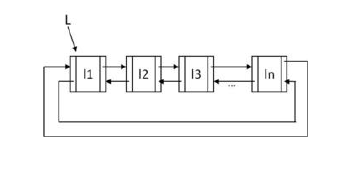
\includegraphics[width=0.4\linewidth]{list.png}\\
Figura 1. Lista circular doblemente enlazada
\end{center}

\subsubsection*{Atributos}
\begin{itemize}
    \item $proximo$. Atributo de instancia que guarda una referencia a la próxima canción a sonar
    \item $numero\_nodos$. Atributo de instancia que indica la cantidad de canciones en la lista de reproducción.
\end{itemize}

\subsubsection*{Métodos}
\begin{itemize}
    \item $\_\_init\_\_(self)$. Constructor de la clase. Crea un lista vacía donde \textit{proximo} sería \texttt{None} y \textit{numero\_nodos} sería \texttt{0}. 
    \item $agregar(self,cancion)$. Inserta un nuevo objeto de la clase Cancion en la posición anterior donde esté apuntado el atributo \textit{proximo} de la lista. Además, el atributo \textit{proximo} referenciaría a ese nuevo nodo. En la figura 3 puede ver como queda la lista de la figura 2 después de agregar.
    \item $agregar\_final(self,cancion)$. Inserta un nuevo objeto de la clase Cancion justo antes del nodo \textit{proximo} de la lista. En la figura 4 puede ver como queda la lista de la figura 2 después de agregar.
    \item $ordenar\_titulo(self)$. Ordena las canciones de la lista de reproducción por título, usando el método \textit{es\_menor\_titulo} de comparación de la clase Cancion con el algoritmo de ordenamiento \textit{Mergesort}. El ordenamiento es sobre la misma lista, no se usan estructuras auxiliares.
    \item $ordenar\_artista(self)$. Ordena las canciones de la lista de reproducción por artista, usando el método \textit{es\_menor\_artista} de comparación de la clase Cancion con el algoritmo de ordenamiento \textit{Mergesort}. El ordenamiento es sobre la misma lista, no se usan estructuras auxiliares.
    \item $eliminar(self,tituloCancion)$. Elimina la canción de la lista cuyo título sea igual al título de tipo \textit{String} pasado como parámetro.
\end{itemize}

Cabe destacar que la lista no puede tener canciones repetidas, es decir, no debe existir ningún par de canciones que al momento de compararlas con el método \textit{es\_igual} retorne \texttt{True}.

\begin{center}
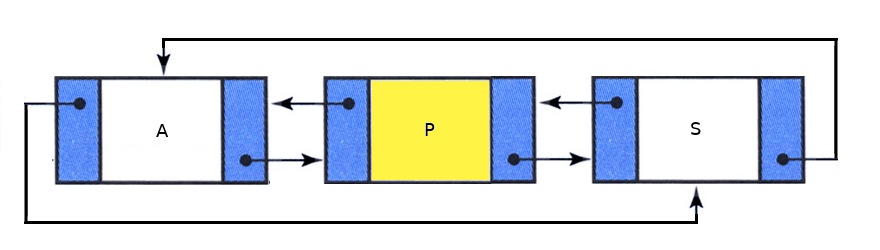
\includegraphics[width=0.5\linewidth]{dlist1.jpg}\\
Figura 2. Lista circular doblemente enlazada. El nodo resaltado es el nodo apuntado.
\end{center}

\begin{center}
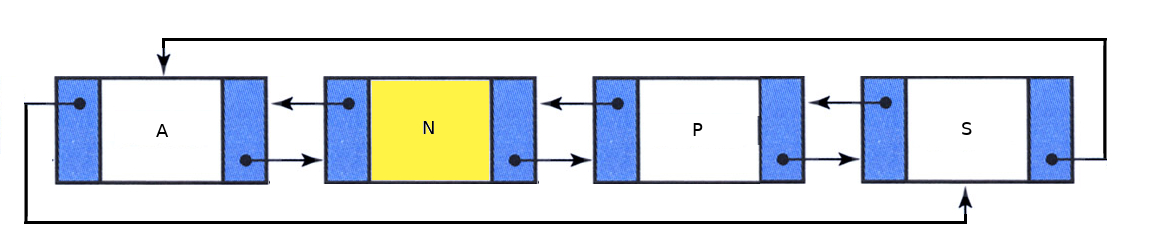
\includegraphics[width=0.6\linewidth]{dlist2.jpg}\\
Figura 3. Lista circular doblemente enlazada despues de agregar con el método \textit{agregar}
\end{center}

\begin{center}
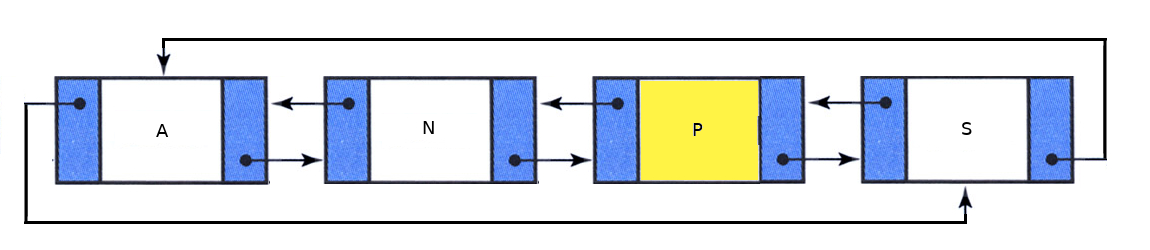
\includegraphics[width=0.6\linewidth]{dlist3.jpg}\\
Figura 4. Lista circular doblemente enlazada después de agregar con el método \textit{agregar\_final}
\end{center}

\subsection*{TAD NodoLista}
El TAD lista de reproducción usará una clase para representar los nodos, esta se encuentra implementada y suministrada junto al enunciado.

\begin{center}
\begin{lstlisting}[language=Python,frame=single]
    class NodoLista:
        def __init__(self, e, s, a):
            self.elemento = e
            self.siguiente = s
            self.anterior = a  
\end{lstlisting}
\end{center}

\section*{TAD Reproductor}
TAD ubicado en el archivo \texttt{reproductor.py}. A pesar de que no implementará ninguna interfaz gráfica, deberá instalar la librería PyQt5, en específico se usarán los módulos PyQt5.QtCore, PyQt5.Gui, PyQt5.QtMultimedia y PyQt5.QtWidgets, para correr el proyecto. Son esenciales para que se muestre la ventana donde estará la lista de reproducción y los distintos botones del reproductor.

Aunque no se modifique esta clase, deberá usar dos métodos de ella para manipular la lista de reproducción y que se visualice en la interfaz gráfica. Esos métodos son los siguientes.

\begin{itemize}
    \item $sonarDespues(cancion)$. Agrega una canción justo después de la canción que está sonando actualmente. Este método utiliza el método $agregar$ del TAD Lista de Reproducción.
    \item $sonarAntes(cancion)$. Agrega una canción justo antes de la canción que está sonando actualmente. Este método utiliza el método $agregar\_final$ del TAD Lista de Reproducción.
\end{itemize}

\section*{Módulo Cliente}
El módulo cliente donde el qrchivo se llamará \texttt{cliente.py} será quien use las estructuras antes mencionadas para consolidar el reproductor de música, para ello se deberá implementar un menú por consola con varias opciones para consultar las canciones disponibles y manipular la lista de reproducción, además se tendrá que procesar un archivo de entrada donde estará la información de las canciones que estarán disponibles.

\subsection*{Menú}
El objetivo es que se manipule la aplicación a través de la linea de comandos y por medio de una interfaz gráfica. La última parte ya está implementada, así que se requiere que desarrolle el menú de consola. La ejecución del programa será por medio del comando.

\begin{center}
\$ $python3\ cliente.py\ <archivo>$
\end{center}

En un principio, el menú mostrará las posibles opciones y luego solicitará que se introduzca un número correspondiente a la opción. En caso de no ser una opción válida, se ignorará. El menú sería similar al que se muestra a continuación.

\begin{center}
\begin{lstlisting}[language=Python,frame=single]
    1. Listar canciones
    2. Agregar para sonar justo después de la canción actual 
    3. Agregar para sonar justo antes de la canción actual
    4. Ordenar lista de reproducción por artista
    5. Ordenar lista de reproducción por titulo
    6. Eliminar canción por título
    7. Mostrar opciones
    8. Salir
    
    Escoja una opción:
\end{lstlisting}
\end{center}

La lista de opciones sólo se mostrará al principio y si se solicita como opción. A continuación se detalla cada opción que debe implementar.

\begin{enumerate}
    \item Se deben listar todas las canciones disponibles, en el orden que se encuentren.
    \item Es necesario que el programa le pida al usuario los datos de una canción para luego crear una instancia \texttt{c} de la clase \textbf{Cancion} y agregarla en la lista de reproducción, y de último se llamaría al método de la clase Reproductor\footnote{La clase Reproductor no debe se modificada en ningún sentido, ella usa las clases que se piden en este enunciado} \textit{sonarDespues} que recibe una instancia de la clase \textbf{Cancion}.
    \item Igual que en la opción anterior, a diferencia que se llama al método \textit{sonarAntes}.
    \item Ordena la lista de reproducción por artista.
    \item Ordena la lista de reproducción por título.
    \item Muestra las opciones disponibles.
    \item Salir del reproductor.
\end{enumerate}

\subsection*{Archivo de entrada}
El archivo de entrada tendrá un formato donde la primero linea corresponde al número de canciones en el archivo, las próximas \texttt{n} linea contendrán un \textit{string} compuesto por el nombre del artista, el titulo de la canción y la dirección del archivo de música y entre ellos existirá un caracter tabulador para separarlos. Puede darse el caso donde exista un salto de linea al final del \textit{string}, el cual no pertenece a la dirección del archivo. A continuación se muestra el formato.

\begin{center}
\begin{lstlisting}[language=Python,frame=single]
    n
    <artista>[TAB]<titulo>[TAB]<direccion de archivo>
    <artista>[TAB]<titulo>[TAB]<direccion de archivo>
    <artista>[TAB]<titulo>[TAB]<direccion de archivo>
    ...
    <artista>[TAB]<titulo>[TAB]<direccion de archivo>
\end{lstlisting}
\end{center}

Deberá leer cada linea, instanciar la clase Cancion e ir almacenándolas en un \textit{ArrayT}. Así se tendrán a disposición todas las canciones de lista de reproducción.

\section*{Condiciones de entrega}
Su programa debe poderse ejecutarse en Python 3 en el sistema de operación \texttt{Linux}. Si un programa no se ejecuta, el equipo tiene cero como nota del proyecto. El trabajo es por equipos de laboratorio. Debe entregar los códigos fuentes de sus programas, en un archivo comprimido llamado Proyecto2-X-Y.tar.gz donde X y Y son los números de carné de los integrantes del grupo. La entrega se realizará por medio del aula virtual antes de la 11:59 pm del sabado 18 de Marzo de 2017. Cada grupo debe entregar firmada, en el laboratorio de la semana 10, la “Declaración de Autenticidad para Entregas”, cuya plantilla se encuentra en la página del curso. Ambos integrantes del equipo deben trabajar en el proyecto. El no cumplimiento de algunos de los requerimientos podrá resultar en el rechazo de su entrega.



\printbibliography

\end{document}
